\documentclass{article}

\def \lastexercisenumber {21}

% ---------------------------------------------------------------- %
% short package descriptions are copied from
% https://ctan.org/

% ---------------------------------------------------------------- %

% Accept different input encodings
\usepackage[utf8]{inputenc}

% Standard package for selecting font encodings
\usepackage[T1]{fontenc}

% ---------------------------------------------------------------- %

% Multilingual support for Plain TEX or LATEX
\usepackage[ngerman]{babel}

% ---------------------------------------------------------------- %

% Set all page margins to 1.5cm
\usepackage{fullpage}

% Margin adjustment and detection of odd/even pages
\usepackage{changepage}

% Flexible and complete interface to document dimensions
\usepackage{geometry}

% ---------------------------------------------------------------- %
% mathematics

\usepackage{amsmath}  % AMS mathematical facilities for LATEX
\usepackage{amssymb}
\usepackage{amsfonts} % TEX fonts from the American Mathematical Society
\usepackage{amsthm}   % Typesetting theorems (AMS style)

% Mathematical tools to use with amsmath
\usepackage{mathtools}

% Support for using RSFS fonts in maths
\usepackage{mathrsfs}

% Commands to produce dots in math that respect font size
\usepackage{mathdots}

% "Blackboard-style" cm fonts
\usepackage{bbm}

% Typeset in-line fractions in a "nice" way
\usepackage{nicefrac}

% Typeset quotient structures with LATEX
\usepackage{faktor}

% Vector arrows
\usepackage{esvect}

% St Mary Road symbols for theoretical computer science
\usepackage{stmaryrd}

% Three series of mathematical symbols
\usepackage{mathabx}

% ---------------------------------------------------------------- %
% algorithms

% Package for typesetting pseudocode
\usepackage{algpseudocode}

% Typeset source code listings using LATEX
\usepackage{listings}

% Reimplementation of and extensions to LATEX verbatim
\usepackage{verbatim}

% If necessary, please use the following 2 packages locally, but never both.
% This is because the algorithm environment gets defined in both packages, which leads to name conflicts.
% \usepackage{algorithm2e}
% \usepackage{algorithm}

% ---------------------------------------------------------------- %
% utilities

% A generic document command parser
\usepackage{xparse}

% Extended conditional commands
\usepackage{xifthen}

% e-TEX tools for LATEX
\usepackage{etoolbox}

% Define commands with suffixes
\usepackage{suffix}

% Extensive support for hypertext in LATEX
\usepackage{hyperref}

% Driver-independent color extensions for LATEX and pdfLATEX
\usepackage{xcolor}

% ---------------------------------------------------------------- %
% graphics

% -------------------------------- %

\usepackage{tikz}

% MISC
\usetikzlibrary{patterns}
\usetikzlibrary{decorations.markings}
\usetikzlibrary{positioning}
\usetikzlibrary{arrows}
\usetikzlibrary{arrows.meta}
\usetikzlibrary{overlay-beamer-styles}

% finite state machines
\usetikzlibrary{automata}

% turing machines
\usetikzlibrary{calc}
\usetikzlibrary{chains}
\usetikzlibrary{decorations.pathmorphing}

% -------------------------------- %

% Draw tree structures
\usepackage[noeepic]{qtree}

% Enhanced support for graphics
\usepackage{graphicx}

% Figures broken into subfigures
\usepackage{subfig}

% Improved interface for floating objects
\usepackage{float}

% Control float placement
\usepackage{placeins}

% Include PDF documents in LATEX
\usepackage{pdfpages}

% ---------------------------------------------------------------- %

% Control layout of itemize, enumerate, description
\usepackage[inline]{enumitem}

% Intermix single and multiple columns
\usepackage{multicol}
\setlength{\columnsep}{1cm}

% Coloured boxes, for LATEX examples and theorems, etc
\usepackage{tcolorbox}

% ---------------------------------------------------------------- %
% tables

% Tabulars with adjustable-width columns
\usepackage{tabularx}

% Tabular column heads and multilined cells
\usepackage{makecell}

% Publication quality tables in LATEX
\usepackage{booktabs}

% ---------------------------------------------------------------- %
% bibliography and quoting

% Sophisticated Bibliographies in LATEX
\usepackage[backend = biber, style = alphabetic]{biblatex}

% Context sensitive quotation facilities
\usepackage{csquotes}

% ---------------------------------------------------------------- %

% ---------------------------------------------------------------- %
% special letters

\newcommand{\N}{\mathbb N}
\newcommand{\Z}{\mathbb Z}
\newcommand{\Q}{\mathbb Q}
\newcommand{\R}{\mathbb R}
\newcommand{\C}{\mathbb C}
\newcommand{\K}{\mathbb K}
\newcommand{\T}{\mathbb T}
\newcommand{\E}{\mathbb E}
\newcommand{\V}{\mathbb V}
\renewcommand{\S}{\mathbb S}
\renewcommand{\P}{\mathbb P}
\newcommand{\1}{\mathbbm 1}
\newcommand{\G}{\mathbb G}

\newcommand{\iu}{\mathrm i}

% ---------------------------------------------------------------- %
% quantors

\newcommand{\Forall}        {\forall ~}
\newcommand{\Exists}        {\exists ~}
\newcommand{\nExists}       {\nexists ~}
\newcommand{\ExistsOnlyOne} {\exists! ~}
\newcommand{\nExistsOnlyOne}{\nexists! ~}
\newcommand{\ForAlmostAll}  {\forall^\infty ~}

% ---------------------------------------------------------------- %
% graphics boxed

\newcommand
{\includegraphicsboxed}
[2][0.75]
{
    \begin{center}
        \begin{tcolorbox}[standard jigsaw, opacityback = 0]

            \centering
            \includegraphics[width = #1 \textwidth]{#2}

        \end{tcolorbox}
    \end{center}
}

\newcommand
{\includegraphicsunboxed}
[2][0.75]
{
    \begin{center}
        \includegraphics[width = #1 \textwidth]{#2}
    \end{center}
}

\NewDocumentCommand
{\includegraphicsgraphicsboxed}
{ O{0.75} O{0.25} m m}
{
    \begin{center}
        \begin{tcolorbox}[standard jigsaw, opacityback = 0]

            \centering
            \includegraphics[width = #1 \textwidth]{#3} \\
            \vspace{#2 cm}
            \includegraphics[width = #1 \textwidth]{#4}

        \end{tcolorbox}
    \end{center}
}

\NewDocumentCommand
{\includegraphicsgraphicsunboxed}
{ O{0.75} O{0.25} m m}
{
    \begin{center}

        \centering
        \includegraphics[width = #1 \textwidth]{#3} \\
        \vspace{#2 cm}
        \includegraphics[width = #1 \textwidth]{#4}

    \end{center}
}

% ---------------------------------------------------------------- %
% braces

\newcommand{\pbraces}[1]{{\left  ( #1 \right  )}}
\newcommand{\bbraces}[1]{{\left  [ #1 \right  ]}}
\newcommand{\Bbraces}[1]{{\left \{ #1 \right \}}}
\newcommand{\vbraces}[1]{{\left  | #1 \right  |}}
\newcommand{\Vbraces}[1]{{\left \| #1 \right \|}}

\newcommand{\abraces}[1]{{\left \langle #1 \right \rangle}}

\newcommand{\floorbraces}[1]{{\left \lfloor #1 \right \rfloor}}
\newcommand{\ceilbraces} [1]{{\left \lceil  #1 \right \rceil }}

\newcommand{\dbbraces}    [1]{{\llbracket     #1 \rrbracket}}
\newcommand{\dpbraces}    [1]{{\llparenthesis #1 \rrparenthesis}}
\newcommand{\dfloorbraces}[1]{{\llfloor       #1 \rrfloor}}
\newcommand{\dceilbraces} [1]{{\llceil        #1 \rrceil}}

\newcommand{\dabraces}[1]{{\left \langle \left \langle #1 \right \rangle \right \rangle}}

\newcommand{\abs}  [1]{\vbraces{#1}}
\newcommand{\round}[1]{\bbraces{#1}}
\newcommand{\floor}[1]{\floorbraces{#1}}
\newcommand{\ceil} [1]{\ceilbraces{#1}}

% ---------------------------------------------------------------- %

% MISC

% metric spaces
\newcommand{\norm}[2][]{\Vbraces{#2}_{#1}}
\DeclareMathOperator{\metric}{d}
\DeclareMathOperator{\dist}  {dist}
\DeclareMathOperator{\diam}  {diam}

% O-notation
\newcommand{\landau}{{\scriptstyle \mathcal{O}}}
\newcommand{\Landau}{\mathcal{O}}

% ---------------------------------------------------------------- %

% math operators

% hyperbolic trigonometric function inverses
\DeclareMathOperator{\areasinh}{areasinh}
\DeclareMathOperator{\areacosh}{areacosh}
\DeclareMathOperator{\areatanh}{areatanh}

% special functions
\DeclareMathOperator{\id} {id}
\DeclareMathOperator{\sgn}{sgn}
\DeclareMathOperator{\Inv}{Inv}
\DeclareMathOperator{\erf}{erf}
\DeclareMathOperator{\pv} {pv}

% exponential function as power
\WithSuffix \newcommand \exp* [1]{\mathrm{e}^{#1}}

% operations on sets
\DeclareMathOperator{\meas}{meas}
\DeclareMathOperator{\card}{card}
\DeclareMathOperator{\Span}{span}
\DeclareMathOperator{\conv}{conv}
\DeclareMathOperator{\cof}{cof}
\DeclareMathOperator{\mean}{mean}
\DeclareMathOperator{\avg}{avg}
\DeclareMathOperator*{\argmax}{argmax}
\DeclareMathOperator*{\argsmax}{argsmax}

% number theory stuff
\DeclareMathOperator{\ggT}{ggT}
\DeclareMathOperator{\kgV}{kgV}
\DeclareMathOperator{\modulo}{mod}

% polynomial stuff
\DeclareMathOperator{\ord}{ord}
\DeclareMathOperator{\grad}{grad}

% function properties
\DeclareMathOperator{\ran}{ran}
\DeclareMathOperator{\supp}{supp}
\DeclareMathOperator{\graph}{graph}
\DeclareMathOperator{\dom}{dom}
\DeclareMathOperator{\Def}{def}
\DeclareMathOperator{\rg}{rg}

% matrix stuff
\DeclareMathOperator{\GL}{GL}
\DeclareMathOperator{\SL}{SL}
\DeclareMathOperator{\U}{U}
\DeclareMathOperator{\SU}{SU}
\DeclareMathOperator{\PSU}{PSU}
% \DeclareMathOperator{\O}{O}
% \DeclareMathOperator{\PO}{PO}
% \DeclareMathOperator{\PSO}{PSO}
\DeclareMathOperator{\diag}{diag}

% algebra stuff
\DeclareMathOperator{\At}{At}
\DeclareMathOperator{\Ob}{Ob}
\DeclareMathOperator{\Hom}{Hom}
\DeclareMathOperator{\End}{End}
\DeclareMathOperator{\Aut}{Aut}
\DeclareMathOperator{\Lin}{L}

% other function classes
\DeclareMathOperator{\Lip}{Lip}
\DeclareMathOperator{\Mod}{Mod}
\DeclareMathOperator{\Dil}{Dil}

% constants
\DeclareMathOperator{\NIL}{NIL}
\DeclareMathOperator{\eps}{eps}

% ---------------------------------------------------------------- %
% doubble & tripple powers

\newcommand
{\primeprime}
{{\prime \prime}}

\newcommand
{\primeprimeprime}
{{\prime \prime \prime}}

\newcommand
{\astast}
{{\ast \ast}}

\newcommand
{\astastast}
{{\ast \ast \ast}}

% ---------------------------------------------------------------- %
% derivatives

\NewDocumentCommand
{\derivative}
{ O{} O{} m m}
{
    \frac
    {\mathrm d^{#2} {#1}}
    {\mathrm d {#3}^{#2}}
}

\NewDocumentCommand
{\pderivative}
{ O{} O{} m m}
{
    \frac
    {\partial^{#2} {#1}}
    {\partial {#3}^{#2}}
}

\DeclareMathOperator{\Div}{div}
\DeclareMathOperator{\rot}{rot}

% ---------------------------------------------------------------- %
% integrals

\NewDocumentCommand
{\Int}
{ O{} O{} m m}
{\int_{#1}^{#2} #3 ~ \mathrm d #4}

\NewDocumentCommand
{\Iint}
{ O{} O{} m m m}
{\iint_{#1}^{#2} #3 ~ \mathrm d #4 ~ \mathrm d #5}

\NewDocumentCommand
{\Iiint}
{ O{} O{} m m m m}
{\iiint_{#1}^{#2} #3 ~ \mathrm d #4 ~ \mathrm d #5 ~ \mathrm d #6}

\NewDocumentCommand
{\Iiiint}
{ O{} O{} m m m m m}
{\iiiint_{#1}^{#2} #3 ~ \mathrm d #4 ~ \mathrm d #5 ~ \mathrm d #6 ~ \mathrm d #7}

\NewDocumentCommand
{\Idotsint}
{ O{} O{} m m m}
{\idotsint_{#1}^{#2} #3 ~ \mathrm d #4 \dots ~ \mathrm d #5}

\NewDocumentCommand
{\Oint}
{ O{} O{} m m}
{\oint_{#1}^{#2} #3 ~ \mathrm d #4}

% ---------------------------------------------------------------- %

% source:
% https://tex.stackexchange.com/questions/203257/tikz-chains-with-one-side-of-the-leftmost-node-thickbold

% #1 (optional): current state, e.g. $q_0$
% #2: cursor position, e.g. 1
% #3: number of displayed cells, e.g. 5
% #4: contents of cells, e.g. {$\triangleright$, $x_1$, \dots, $x_n$, \textvisiblespace}

\newcommand{\turingtape}[4][]
{
    \begin{tikzpicture}

        \tikzset{tape/.style={minimum size=.7cm, draw}}

        \begin{scope}[start chain=0 going right, node distance=0mm]
            \foreach \x [count=\i] in #4
            {
                \ifnum\i=#3 % if last node reset outer sep to 0pt
                    \node [on chain=0, tape, outer sep=0pt] (n\i) {\x};
                    \draw (n\i.north east) -- ++(.1,0) decorate [decoration={zigzag, segment length=.12cm, amplitude=.02cm}] {-- ($(n\i.south east)+(+.1,0)$)} -- (n\i.south east) -- cycle;
                \else
                    \node [on chain=0, tape] (n\i) {\x};
                \fi

                \ifnum\i=1 % if first node draw a thick line at the left
                    \draw [line width=.1cm] (n\i.north west) -- (n\i.south west);
                \fi
            }
 
            \node [right=.25cm of n#3] {$\cdots$};
            \node [tape, above left=.25cm and 1cm of n1] (q) {#1};
            \draw [>=latex, ->] (q) -| (n#2);

        \end{scope}

    \end{tikzpicture}
}

% ---------------------------------------------------------------- %

% ---------------------------------------------------------------- %
% amsthm-environments:

\theoremstyle{definition}

% numbered theorems
\newtheorem{theorem}             {Satz}[section]
\newtheorem{lemma}      [theorem]{Lemma}
\newtheorem{corollary}  [theorem]{Korollar}
\newtheorem{proposition}[theorem]{Proposition}
\newtheorem{remark}     [theorem]{Bemerkung}
\newtheorem{definition} [theorem]{Definition}
\newtheorem{example}    [theorem]{Beispiel}
\newtheorem{heuristics} [theorem]{Heuristik}

% unnumbered theorems
\newtheorem*{theorem*}    {Satz}
\newtheorem*{lemma*}      {Lemma}
\newtheorem*{corollary*}  {Korollar}
\newtheorem*{proposition*}{Proposition}
\newtheorem*{remark*}     {Bemerkung}
\newtheorem*{definition*} {Definition}
\newtheorem*{example*}    {Beispiel}
\newtheorem*{heuristics*} {Heuristik}

% ---------------------------------------------------------------- %
% exercise- and solution-environments:

% Please define this stuff in project ("main.tex"):
% \def \lastexercisenumber {...}

\newtheorem{exercise}{Aufgabe}
\setcounter{exercise}{\lastexercisenumber}

\newenvironment{solution}
{
  \begin{proof}[Lösung]
}{
  \end{proof}
}

% ---------------------------------------------------------------- %
% MISC translations for environment-names

\renewcommand{\proofname} {Beweis}
\renewcommand{\figurename}{Abbildung}
\renewcommand{\tablename} {Tabelle}

% ---------------------------------------------------------------- %

% ---------------------------------------------------------------- %
% https://www.overleaf.com/learn/latex/Code_listing

\definecolor{codegreen} {rgb}{0, 0.6, 0}
\definecolor{codegray}    {rgb}{0.5, 0.5, 0.5}
\definecolor{codepurple}{rgb}{0.58, 0, 0.82}
\definecolor{backcolour}{rgb}{0.95, 0.95, 0.92}

\lstdefinestyle{overleaf}
{
    backgroundcolor = \color{backcolour},
    commentstyle = \color{codegreen},
    keywordstyle = \color{magenta},
    numberstyle = \tiny\color{codegray},
    stringstyle = \color{codepurple},
    basicstyle = \ttfamily \footnotesize,
    breakatwhitespace = false,
    breaklines = true,
    captionpos = b,
    keepspaces = true,
    numbers = left,
    numbersep = 5pt,
    showspaces = false,
    showstringspaces = false,
    showtabs = false,
    tabsize = 2
}

% ---------------------------------------------------------------- %
% https://en.wikibooks.org/wiki/LaTeX/Source_Code_Listings

\lstdefinestyle{customc}
{
    belowcaptionskip = 1 \baselineskip,
    breaklines = true,
    frame = L,
    xleftmargin = \parindent,
    language = C,
    showstringspaces = false,
    basicstyle = \footnotesize \ttfamily,
    keywordstyle = \bfseries \color{green!40!black},
    commentstyle = \itshape \color{purple!40!black},
    identifierstyle = \color{blue},
    stringstyle = \color{orange},
}

\lstdefinestyle{customasm}
{
    belowcaptionskip = 1 \baselineskip,
    frame = L,
    xleftmargin = \parindent,
    language = [x86masm] Assembler,
    basicstyle = \footnotesize\ttfamily,
    commentstyle = \itshape\color{purple!40!black},
}

% ---------------------------------------------------------------- %
% https://tex.stackexchange.com/questions/235731/listings-syntax-for-literate

\definecolor{maroon}        {cmyk}{0, 0.87, 0.68, 0.32}
\definecolor{halfgray}      {gray}{0.55}
\definecolor{ipython_frame} {RGB}{207, 207, 207}
\definecolor{ipython_bg}    {RGB}{247, 247, 247}
\definecolor{ipython_red}   {RGB}{186, 33, 33}
\definecolor{ipython_green} {RGB}{0, 128, 0}
\definecolor{ipython_cyan}  {RGB}{64, 128, 128}
\definecolor{ipython_purple}{RGB}{170, 34, 255}

\lstdefinestyle{stackexchangePython}
{
    breaklines = true,
    %
    extendedchars = true,
    literate =
    {á}{{\' a}} 1 {é}{{\' e}} 1 {í}{{\' i}} 1 {ó}{{\' o}} 1 {ú}{{\' u}} 1
    {Á}{{\' A}} 1 {É}{{\' E}} 1 {Í}{{\' I}} 1 {Ó}{{\' O}} 1 {Ú}{{\' U}} 1
    {à}{{\` a}} 1 {è}{{\` e}} 1 {ì}{{\` i}} 1 {ò}{{\` o}} 1 {ù}{{\` u}} 1
    {À}{{\` A}} 1 {È}{{\' E}} 1 {Ì}{{\` I}} 1 {Ò}{{\` O}} 1 {Ù}{{\` U}} 1
    {ä}{{\" a}} 1 {ë}{{\" e}} 1 {ï}{{\" i}} 1 {ö}{{\" o}} 1 {ü}{{\" u}} 1
    {Ä}{{\" A}} 1 {Ë}{{\" E}} 1 {Ï}{{\" I}} 1 {Ö}{{\" O}} 1 {Ü}{{\" U}} 1
    {â}{{\^ a}} 1 {ê}{{\^ e}} 1 {î}{{\^ i}} 1 {ô}{{\^ o}} 1 {û}{{\^ u}} 1
    {Â}{{\^ A}} 1 {Ê}{{\^ E}} 1 {Î}{{\^ I}} 1 {Ô}{{\^ O}} 1 {Û}{{\^ U}} 1
    {œ}{{\oe}}  1 {Œ}{{\OE}}  1 {æ}{{\ae}}  1 {Æ}{{\AE}}  1 {ß}{{\ss}}  1
    {ç}{{\c c}} 1 {Ç}{{\c C}} 1 {ø}{{\o}} 1 {å}{{\r a}} 1 {Å}{{\r A}} 1
    {€}{{\EUR}} 1 {£}{{\pounds}} 1
}


% Python definition (c) 1998 Michael Weber
% Additional definitions (2013) Alexis Dimitriadis
% modified by me (should not have empty lines)

\lstdefinelanguage{iPython}{
    morekeywords = {access, and, break, class, continue, def, del, elif, else, except, exec, finally, for, from, global, if, import, in, is, lambda, not, or, pass, print, raise, return, try, while}, %
    %
    % Built-ins
    morekeywords = [2]{abs, all, any, basestring, bin, bool, bytearray, callable, chr, classmethod, cmp, compile, complex, delattr, dict, dir, divmod, enumerate, eval, execfile, file, filter, float, format, frozenset, getattr, globals, hasattr, hash, help, hex, id, input, int, isinstance, issubclass, iter, len, list, locals, long, map, max, memoryview, min, next, object, oct, open, ord, pow, property, range, raw_input, reduce, reload, repr, reversed, round, set, setattr, slice, sorted, staticmethod, str, sum, super, tuple, type, unichr, unicode, vars, xrange, zip, apply, buffer, coerce, intern}, %
    %
    sensitive = true, %
    morecomment = [l] \#, %
    morestring = [b]', %
    morestring = [b]", %
    %
    morestring = [s]{'''}{'''}, % used for documentation text (mulitiline strings)
    morestring = [s]{"""}{"""}, % added by Philipp Matthias Hahn
    %
    morestring = [s]{r'}{'},     % `raw' strings
    morestring = [s]{r"}{"},     %
    morestring = [s]{r'''}{'''}, %
    morestring = [s]{r"""}{"""}, %
    morestring = [s]{u'}{'},     % unicode strings
    morestring = [s]{u"}{"},     %
    morestring = [s]{u'''}{'''}, %
    morestring = [s]{u"""}{"""}, %
    %
    % {replace}{replacement}{lenght of replace}
    % *{-}{-}{1} will not replace in comments and so on
    literate = 
    {á}{{\' a}} 1 {é}{{\' e}} 1 {í}{{\' i}} 1 {ó}{{\' o}} 1 {ú}{{\' u}} 1
    {Á}{{\' A}} 1 {É}{{\' E}} 1 {Í}{{\' I}} 1 {Ó}{{\' O}} 1 {Ú}{{\' U}} 1
    {à}{{\` a}} 1 {è}{{\` e}} 1 {ì}{{\` i}} 1 {ò}{{\` o}} 1 {ù}{{\` u}} 1
    {À}{{\` A}} 1 {È}{{\' E}} 1 {Ì}{{\` I}} 1 {Ò}{{\` O}} 1 {Ù}{{\` U}} 1
    {ä}{{\" a}} 1 {ë}{{\" e}} 1 {ï}{{\" i}} 1 {ö}{{\" o}} 1 {ü}{{\" u}} 1
    {Ä}{{\" A}} 1 {Ë}{{\" E}} 1 {Ï}{{\" I}} 1 {Ö}{{\" O}} 1 {Ü}{{\" U}} 1
    {â}{{\^ a}} 1 {ê}{{\^ e}} 1 {î}{{\^ i}} 1 {ô}{{\^ o}} 1 {û}{{\^ u}} 1
    {Â}{{\^ A}} 1 {Ê}{{\^ E}} 1 {Î}{{\^ I}} 1 {Ô}{{\^ O}} 1 {Û}{{\^ U}} 1
    {œ}{{\oe}}  1 {Œ}{{\OE}}  1 {æ}{{\ae}}  1 {Æ}{{\AE}}  1 {ß}{{\ss}}  1
    {ç}{{\c c}} 1 {Ç}{{\c C}} 1 {ø}{{\o}} 1 {å}{{\r a}} 1 {Å}{{\r A}} 1
    {€}{{\EUR}} 1 {£}{{\pounds}} 1
    %
    {^}{{{\color{ipython_purple}\^ {}}}} 1
    { = }{{{\color{ipython_purple} = }}} 1
    %
    {+}{{{\color{ipython_purple}+}}} 1
    {*}{{{\color{ipython_purple}$^\ast$}}} 1
    {/}{{{\color{ipython_purple}/}}} 1
    %
    {+=}{{{+=}}} 1
    {-=}{{{-=}}} 1
    {*=}{{{$^\ast$ = }}} 1
    {/=}{{{/=}}} 1,
    literate = 
    *{-}{{{\color{ipython_purple} -}}} 1
     {?}{{{\color{ipython_purple} ?}}} 1,
    %
    identifierstyle = \color{black}\ttfamily,
    commentstyle = \color{ipython_cyan}\ttfamily,
    stringstyle = \color{ipython_red}\ttfamily,
    keepspaces = true,
    showspaces = false,
    showstringspaces = false,
    %
    rulecolor = \color{ipython_frame},
    frame = single,
    frameround = {t}{t}{t}{t},
    framexleftmargin = 6mm,
    numbers = left,
    numberstyle = \tiny\color{halfgray},
    %
    %
    backgroundcolor = \color{ipython_bg},
    % extendedchars = true,
    basicstyle = \scriptsize,
    keywordstyle = \color{ipython_green}\ttfamily,
}

% ---------------------------------------------------------------- %
% https://tex.stackexchange.com/questions/417884/colour-r-code-to-match-knitr-theme-using-listings-minted-or-other

\geometry{verbose, tmargin = 2.5cm, bmargin = 2.5cm, lmargin = 2.5cm, rmargin = 2.5cm}

\definecolor{backgroundCol}  {rgb}{.97, .97, .97}
\definecolor{commentstyleCol}{rgb}{0.678, 0.584, 0.686}
\definecolor{keywordstyleCol}{rgb}{0.737, 0.353, 0.396}
\definecolor{stringstyleCol} {rgb}{0.192, 0.494, 0.8}
\definecolor{NumCol}         {rgb}{0.686, 0.059, 0.569}
\definecolor{basicstyleCol}  {rgb}{0.345, 0.345, 0.345}

\lstdefinestyle{stackexchangeR}
{
    language = R,                                        % the language of the code
    basicstyle = \small \ttfamily \color{basicstyleCol}, % the size of the fonts that are used for the code
    % numbers = left,                                      % where to put the line-numbers
    numberstyle = \color{green},                         % the style that is used for the line-numbers
    stepnumber = 1,                                      % the step between two line-numbers. If it is 1, each line will be numbered
    numbersep = 5pt,                                     % how far the line-numbers are from the code
    backgroundcolor = \color{backgroundCol},             % choose the background color. You must add \usepackage{color}
    showspaces = false,                                  % show spaces adding particular underscores
    showstringspaces = false,                            % underline spaces within strings
    showtabs = false,                                    % show tabs within strings adding particular underscores
    % frame = single,                                      % adds a frame around the code
    % rulecolor = \color{white},                           % if not set, the frame-color may be changed on line-breaks within not-black text (e.g. commens (green here))
    tabsize = 2,                                         % sets default tabsize to 2 spaces
    captionpos = b,                                      % sets the caption-position to bottom
    breaklines = true,                                   % sets automatic line breaking
    breakatwhitespace = false,                           % sets if automatic breaks should only happen at whitespace
    keywordstyle = \color{keywordstyleCol},              % keyword style
    commentstyle = \color{commentstyleCol},              % comment style
    stringstyle = \color{stringstyleCol},                % string literal style
    literate = %
    *{0}{{{\color{NumCol} 0}}} 1
     {1}{{{\color{NumCol} 1}}} 1
     {2}{{{\color{NumCol} 2}}} 1
     {3}{{{\color{NumCol} 3}}} 1
     {4}{{{\color{NumCol} 4}}} 1
     {5}{{{\color{NumCol} 5}}} 1
     {6}{{{\color{NumCol} 6}}} 1
     {7}{{{\color{NumCol} 7}}} 1
     {8}{{{\color{NumCol} 8}}} 1
     {9}{{{\color{NumCol} 9}}} 1
}

% ---------------------------------------------------------------- %
% Fundament Mathematik

\lstdefinestyle{fundament}{basicstyle = \ttfamily}

% ---------------------------------------------------------------- %


\addbibresource{../../../../Fundament-LaTeX/references.bib}

\graphicspath{{../../../../Fundament-LaTeX/images/}}

\parskip 0pt
\parindent 0pt

\title
{
    Reinforcement Learning \\
    \vspace{4pt}
    \normalsize
    \textit{3. Übung}
}
\author{Richard Weiss}
\date{3.5.2021}

\begin{document}

\maketitle

% --------------------------------------------------------------------------------

\begin{exercise}[Exercise 4.1]

In Example 4.1, if $\pi$ is the equiprobable random policy, what is $q_\pi(11, \mathit{down})$?

\begin{figure}[H]
    \centering
    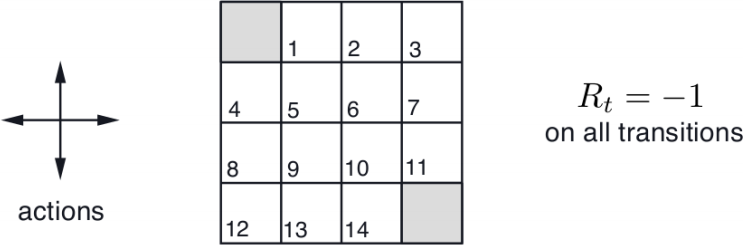
\includegraphics[width = 0.5 \textwidth]{3.22.png}
    \caption{Example 4.1}
    \label{fig:3.22.1}
\end{figure}

\end{exercise}

% --------------------------------------------------------------------------------

\begin{solution}

Let $\infty$ denote the lower right terminal state.
$v_\pi$ has already been calculated in Figure 4.1 from \cite*[page 77]{SuttonRichardS2018Rl:a}.
We only have to apply (4.6) from \cite*[page 78]{SuttonRichardS2018Rl:a}

\begin{align*}
    q_\pi(11, \mathit{down})
    & =
    \sum_{s^\prime, r}
        p(s^\prime, r \mid 11, \mathit{down})
        \bbraces{r + v_\pi(s^\prime)} \\
    & =
    p(\infty, -1 \mid 11, \mathit{down})
    \bbraces{-1 + v_\pi(\infty)} \\
    & =
    1 [-1 + 0] \\
    & =
    -1
\end{align*}

\end{solution}

% --------------------------------------------------------------------------------

% --------------------------------------------------------------------------------

\begin{exercise}

In Example 4.1, suppose a new state $15$ is added to the gridworld just below state $13$, and its actions, $\mathit{left}, \mathit{up}$ $\mathit{right}$, and $\mathit{down}$, take the agent to states $12$, $13$, $14$, and $15$, respectively.
Assume that the transistions from the original states are unchnged. 
What, the, ist $v_\pi(15)$ for the equiprobable random policy?
Now suppose the dynamics of state $13$ are also changed, such that action down from state $13$ takes the agent to the new state $15$.
What is $v_\pi(15)$ for the equiprobable random policy in this case?

\end{exercise}

% --------------------------------------------------------------------------------

\begin{solution}

\phantom{}

\begin{enumerate}[label = \arabic*.]

    \item Part:
    
    We formally define

    \begin{align*}
        \mathcal A(15)
        :=
        \Bbraces
        {
            \mathit{left},
            \mathit{up},
            \mathit{right},
            \mathit{down}
        }.
    \end{align*}

    Now, we know that the Bellman equations (3.14), from \cite*[page 59]{SuttonRichardS2018Rl:a}, have to apply.

    \begin{align*}
        v_\pi(15)
        & =
        \sum_{a \in \mathcal A(s)}
            \pi(a \mid 15)
            \sum_{\substack{s^\prime \in \mathcal S \cup \Bbraces{15} \\ r \in \mathcal R}}
                p(s^\prime, r \mid 15, a)
                \bbraces{r + \gamma v_\pi(s^\prime)} \\
        & =
        \frac{1}{4}
        (
            -1 + \gamma v_\pi(12)
        )
        +
        \frac{1}{4}
        (
            -1 + \gamma v_\pi(13)
        )
        +
        \frac{1}{4}
        (
            -1 + \gamma v_\pi(14)
        )
        +
        \frac{1}{4}
        (
            -1 + \gamma v_\pi(15)
        ) \\
        & =
        \frac{\gamma}{4}
        (
            v_\pi(12) + v_\pi(13) + v_\pi(14)
        )
        +
        \frac{\gamma}{4}
        v_\pi(15)
        -
        4
        \frac{1}{4}
    \end{align*}

    \begin{align*}
        \iff
        \frac{\gamma}{4}
        (
            v_\pi(12) + v_\pi(13) + v_\pi(14)
        )
        -
        1
        & =
        v_\pi(15) - \frac{\gamma}{4} v_\pi(15) \\
        & =
        \pbraces
        {
            1 - \frac{\gamma}{4}
        }
        v_\pi(15)
    \end{align*}

    \begin{align*}
        \iff
        v_\pi(15)
        & =
        \frac
        {
            \frac{\gamma}{4}
            (
                v_\pi(12) + v_\pi(13) + v_\pi(14)
            )
            -
            1
        }{
            1 - \frac{\gamma}{4}
        } \\
        & =
        \frac
        {
            \gamma (-22 - 20 - 14) - 4
        }{
            4 - \gamma
        } \\
        & =
        \frac{56 \gamma + 4}{\gamma - 4} \\
        & =
        \begin{cases}
            -1,  & \gamma = 0, \\
            -20, & \gamma = 1
        \end{cases}
    \end{align*}

    \begin{figure}[H]
        \centering
        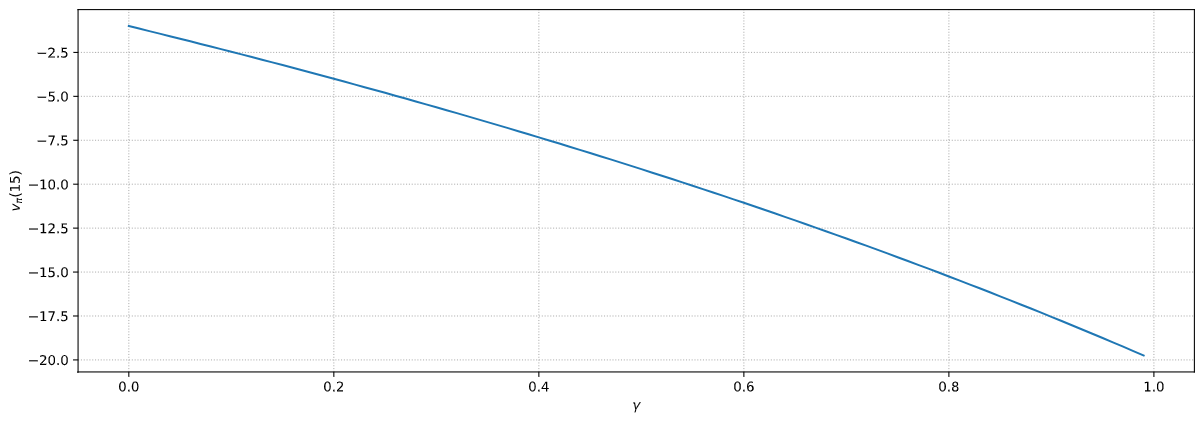
\includegraphics[width = 0.95 \textwidth]{3.23.png}
        \caption{}
        \label{fig:2.23}
    \end{figure}

    \item Part:
    
    \begin{align*}
        v_{\pi, \text{old}}(s)
        & =
        \sum_{a \in \mathcal A(s)}
            \pi(a \mid s)
            \sum_{\substack{s^\prime \in \mathcal S \cup \Bbraces{15} \\ r \in \mathcal R}}
                p_\text{old}(s^\prime, r \mid s, a)
                \bbraces{r + \gamma v_{\pi, \text{old}}(s^\prime)} \\
        & =
        \sum_{a \in \mathcal A(s) \setminus \Bbraces{\mathit{down}}}
            \pi(a \mid s)
            \sum_{\substack{s^\prime \in \mathcal S \cup \Bbraces{15} \\ r \in \mathcal R}}
                p_\text{old}(s^\prime, r \mid s, a)
                \bbraces{r + \gamma v_{\pi, \text{old}}(s^\prime)} \\
        & +
        \pi(\mathit{down} \mid s)
        \sum_{r \in \mathcal R}
            \Bigg (
                \sum_{s^\prime \in \mathcal S \setminus \Bbraces{13}}
                    p_\text{old}(s^\prime, r \mid s, \mathit{down})
                    \bbraces{r + \gamma v_{\pi, \text{old}}(s^\prime)} \\
                & +
                p_\text{old}(13, r \mid s, \mathit{down})
                \bbraces{r + \gamma v_{\pi, \text{old}}(13)}
                +
                p_\text{old}(15, r \mid s, \mathit{down})
                \bbraces{r + \gamma v_{\pi, \text{old}}(15)}
            \Bigg ) \\
        & =
        \sum_{a \in \mathcal A(s) \setminus \Bbraces{\mathit{down}}}
            \pi(a \mid s)
            \sum_{\substack{s^\prime \in \mathcal S \cup \Bbraces{15} \\ r \in \mathcal R}}
                p_\text{old}(s^\prime, r \mid s, a)
                \bbraces{r + \gamma v_{\pi, \text{old}}(s^\prime)} \\
        & +
        \pi(\mathit{down} \mid s)
        \sum_{r \in \mathcal R}
            \Bigg (
                \sum_{s^\prime \in \mathcal S \setminus \Bbraces{13}}
                    p_\text{old}(s^\prime, r \mid s, \mathit{down})
                    \bbraces{r + \gamma v_{\pi, \text{old}}(s^\prime)} \\
                & +
                (
                    p_\text{old}(13, r \mid s, \mathit{down})
                    +
                    p_\text{old}(15, r \mid s, \mathit{down})
                )
                \bbraces{r + \gamma (-20)}
            \Bigg ) \\
        & \stackrel{!}{=}
        \sum_{a \in \mathcal A(s) \setminus \Bbraces{\mathit{down}}}
            \pi(a \mid s)
            \sum_{\substack{s^\prime \in \mathcal S \cup \Bbraces{15} \\ r \in \mathcal R}}
                p_\text{new}(s^\prime, r \mid s, a)
                \bbraces{r + \gamma v_{\pi, \text{new}}(s^\prime)} \\
        & +
        \pi(\mathit{down} \mid s)
        \sum_{r \in \mathcal R}
            \Bigg (
                \sum_{s^\prime \in \mathcal S \setminus \Bbraces{13}}
                    p_\text{new}(s^\prime, r \mid s, \mathit{down})
                    \bbraces{r + \gamma v_{\pi, \text{new}}(s^\prime)} \\
                & +
                (
                    p_\text{new}(13, r \mid s, \mathit{down})
                    +
                    p_\text{new}(15, r \mid s, \mathit{down})
                )
                \bbraces{r + \gamma (-20)}
            \Bigg ) \\
        & \stackrel{!!}{=}
        \sum_{a \in \mathcal A(s) \setminus \Bbraces{\mathit{down}}}
            \pi(a \mid s)
            \sum_{\substack{s^\prime \in \mathcal S \cup \Bbraces{15} \\ r \in \mathcal R}}
                p_\text{new}(s^\prime, r \mid s, a)
                \bbraces{r + \gamma v_{\pi, \text{new}}(s^\prime)} \\
        & +
        \pi(\mathit{down} \mid s)
        \sum_{r \in \mathcal R}
            \Bigg (
                \sum_{s^\prime \in \mathcal S \setminus \Bbraces{13}}
                    p_\text{new}(s^\prime, r \mid s, \mathit{down})
                    \bbraces{r + \gamma v_{\pi, \text{new}}(s^\prime)} \\
                & +
                p_\text{new}(13, r \mid s, \mathit{down})
                \bbraces{r + \gamma v_{\pi, \text{new}}(13)}
                +
                p_\text{new}(15, r \mid s, \mathit{down})
                \bbraces{r + \gamma v_{\pi, \text{new}}(15)}
            \Bigg ) \\
        & =
        \sum_{a \in \mathcal A(s)}
            \pi(a \mid s)
            \sum_{\substack{s^\prime \in \mathcal S \cup \Bbraces{15} \\ r \in \mathcal R}}
                p_\text{new}(s^\prime, r \mid s, a)
                \bbraces{r + \gamma v_{\pi, \text{new}}(s^\prime)} \\
        & =
        v_{\pi, \text{new}}(s)
    \end{align*}

    \blockquote{!} follows from

    \begin{align*}
        p_\text{old}(13, r \mid s, \mathit{down})
        +
        p_\text{old}(15, r \mid s, \mathit{down})
        =
        p_\text{new}(13, r \mid s, \mathit{down})
        +
        p_\text{new}(15, r \mid s, \mathit{down}).
    \end{align*}

    For \blockquote{!} we used the Ansatz $v_{\pi, \text{new}} \doteq v_{\pi, \text{old}}$, which checks out in the end, by virtue of the Bellman equation's unique solvability.

\end{enumerate}

\end{solution}

% --------------------------------------------------------------------------------

% --------------------------------------------------------------------------------

\begin{exercise}[Inplementation Task: $1$-D Gridworld]

Consider the following one-dimensional \enquote{gridworld}:
You are on a route consisting of $10$ states.
The state on the left side is a terminal state with a reward of $+10$ and the state on the right is also a terminal state width a reward of $-5$.
You can move left and right.

\begin{figure}[H]
    \centering
    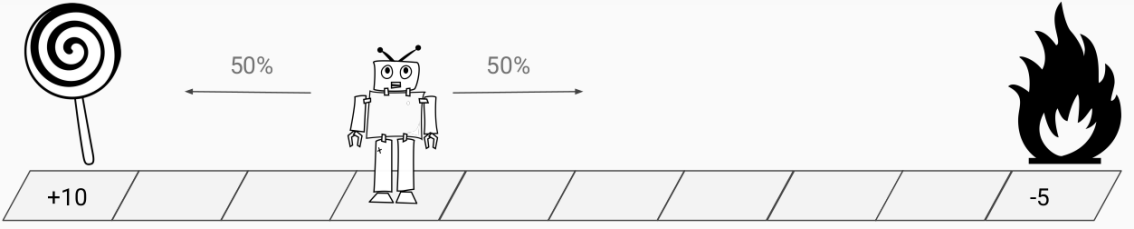
\includegraphics[width = 0.75 \textwidth]{3.24.png}
    \caption{$1$D Gridworld}
    \label{fig:3.24}
\end{figure}

Write an implementation of Dynamic Programming for estimating the values of the above states under the equiprobable random policy.

Then use policy improvement to find the optimal policy.

\end{exercise}

% --------------------------------------------------------------------------------

\begin{solution}

ToDo!

\end{solution}

% --------------------------------------------------------------------------------

% --------------------------------------------------------------------------------

\begin{exercise}[Exercise 4.3]

What are the equations analogous to (4.3), (4.4), and (4.5) for the action-value function $q_\pi$ and its successive approximation by a sequence of functions $q_0$, $q_1$, $q_2$, \dots?
(Textbook p. 74)

\begin{align*} % \label{eq:3.25.1_2}
    v_\pi(s)
    & \doteq
    \E_\pi[G_t \mid S_t = s] \\
    & =
    \E_\pi[R_{t+1} + \gamma G_{t+1} \mid S_t = s] \\
    & =
    \E_\pi[R_{t+1} + \gamma v_\pi(S_{t+1}) \mid S_t = s] \tag{4.3} \\
    & =
    \sum_a
        \pi(a \mid s)
        \sum_{s^\prime, r}
            p(s^\prime, r \mid s, a)
            \bbraces{r + \gamma v_\pi(s^\prime)} \tag{4.4}
\end{align*}

\begin{align*}
    v_{k+1}
    & \doteq
    \E_\pi[R_{t+1} + \gamma v_k(S_{t+1}) \mid S_t = s] \\
    & =
    \sum_a
        \pi(a \mid s)
        \sum_{s^\prime, r}
            p(s^\prime, r \mid s, a)
            \bbraces{r + \gamma v_k(s^\prime)} \tag{4.5}
\end{align*}

\end{exercise}

% --------------------------------------------------------------------------------

\begin{solution}

Recall the results about the Bellman equations for $q_\pi$ from Exercise 3.17.

\begin{align*}
    q_\pi(s, a)
    & =
    \sum_{s^\prime, r}
        p(s^\prime, r \mid s, a)
        \sum_{a^\prime}
            \pi(a^\prime \mid s^\prime)
            \bbraces{r + \gamma q_\pi(s^\prime, a^\prime)} \tag{4.4'} \\
    & =
    \E_\pi[R_{t+1} + \gamma q_\pi(S_{t+1}, A_{t+1}) \mid S_t = s] \tag{4.3'}
\end{align*}

\begin{align*}
    q_{k+1}
    & \doteq
    \sum_{s^\prime, r}
        p(s^\prime, r \mid s, a)
        \sum_{a^\prime}
            \pi(a^\prime \mid s^\prime)
            \bbraces{r + \gamma q_k(s^\prime, a^\prime)} \tag{4.5'} \\
    & =
    \E_\pi[R_{t+1} + \gamma q_k(S_{t+1}, A_{t+1}) \mid S_t = s]
\end{align*}

\end{solution}

% --------------------------------------------------------------------------------

% --------------------------------------------------------------------------------

\begin{exercise}[Exercise 4.5]

How would policy iteration be defined for action values?
Give a complete algorithm for computing $q_\ast$, analogous to that on page 80 for computing $v_\ast$.
Please pay special attention to this exercise, because the ideas involved will be used throughout the rest of the book.

\end{exercise}

% --------------------------------------------------------------------------------

\begin{solution}

Recall, from \cite*[page 79]{SuttonRichardS2018Rl:a}, that

\begin{align*}
    \pi^\prime(s)
    \doteq
    \argmax_a q_\pi(s, a).
\end{align*}

\begin{tcolorbox}[title = Policy Iteration (using iterative policy evaluation) for estimating $\pi \approx \pi_\ast$]

    \begin{enumerate}[label = \arabic*.]

        \item Initialization
        
        \begin{align*}
            & Q(s, a) \in \R ~\text{and}~ \pi(s) \in \mathcal A(s) ~\text{arbitrarily for all}~ s \in \mathcal S ~\text{and}~ a \in \mathcal A(s)            
        \end{align*}

        \item Policy Evaluation
        
        \begin{align*}
            & \text{Loop}: \\
            & \quad \Delta \leftarrow 0 \\
            & \quad \text{Loop for each $s \in \mathcal S$}: \\
            & \quad \quad \text{Loop for each $a \in \mathcal A(s)$}: \\
            & \quad \quad \quad q \leftarrow Q(s, a) \\
            & \quad \quad \quad Q(s, a) \leftarrow \sum_{s^\prime, r} p(s^\prime, r \mid s, a) \sum_{a^\prime} \pi(a^\prime \mid s^\prime) \bbraces{r + \gamma Q(s^\prime, a^\prime)} \\
            & \quad \quad \quad \Delta \leftarrow \max(\Delta, |q - Q(s, a)|) \\
            & \text{until $\Delta < \theta$ (a small positive number determining the accuracy of estimation)}
        \end{align*}

        \item Policy Improvement

        \begin{align*}
            & \textit{policy-stable} \leftarrow \textit{true} \\
            & \text{For each $s \in \mathcal S$}: \\
            & \quad \textit{old-action} \leftarrow \pi(s) \\
            & \quad \pi(s) \leftarrow \argmax_a Q(s, a) \\
            & \quad \text{If $\textit{old-action} \neq \pi(s)$, then $\textit{policy-stable} \leftarrow \textit{false}$} \\
            & \text{If $\textit{policy-stable}$, then stop and return $Q \approx q_\ast$ and $\pi \approx \pi_\ast$; else go to $2$}
        \end{align*}

    \end{enumerate}

\end{tcolorbox}

\end{solution}

% --------------------------------------------------------------------------------

% -------------------------------------------------------------------------------- %

\begin{exercise}

Betrachten Sie die Funktion

\begin{align*}
    f(x)
    =
    \begin{cases}
        1 & 0 \leq |x| \leq d \\
        0 & d \leq |x| \leq \pi
    \end{cases}
\end{align*}

und berechnen Sie damit und Bsp. 25

\begin{align*}
    \sum_{n=1}^\infty
    \frac{\sin^2(n d)}{n^2}
    \quad
    \text{und}
    \quad
    \sum_{n=1}^\infty
    \frac{\cos^2(n d)}{n^2}.
\end{align*}

\end{exercise}

% -------------------------------------------------------------------------------- %

\begin{solution}

\phantom{}

\begin{enumerate}[label = \arabic*.]

    \item Teil (Fourier-Reihe):

    $f = \1_\bbraces{-d, d}$, $d \in [0, \pi]$ ist eine gerade Funktion $\in L^2[-\pi, \pi]$.
    Weil $\sin$ ungerade und $f$ gerade ist, fallen die $\sin$-Terme weg.
    Wir berechnen also nur die $\cos$-Terme.
    
    \begin{align*}
        a_0
        =
        \frac{1}{\pi}
        \Int[-\pi][\pi]{f(x)}{x}
        =
        \frac{1}{\pi}
        \Int[-d][d]{}{x}
        =
        \frac{2 d}{\pi}
    \end{align*}
    
    \begin{multline*}
        a_n
        =
        \frac{1}{\pi}
        \Int[-\pi][\pi]{f(x) \cos(n x)}{x}
        =
        \frac{1}{\pi}
        \Int[-d][d]{\cos(n x)}{x} \\
        =
        \frac{2}{\pi}
        \Int[0][d]{\cos(n x)}{x}
        =
        \frac{2}{\pi}
        \frac{1}{n}
        \Int[0][n d]{\cos u}{u}
        =
        \frac{2}{n \pi}
        \sin u \Big |_{u=0}^{n d}
        =
        \frac{2}{n \pi}
        \sin(n d)
    \end{multline*}
    
    Dabei haben wir folgende Substitution verwendet.
    
    \begin{align*}
        u = n x
        \implies
        \derivative[][u]{x} = n
        \implies
        \mathrm{d} x = \frac{1}{n} \mathrm{d} u
    \end{align*}
    
    \begin{align*}
        \implies
        f(x)
        =
        \frac{a_0}{2}
        +
        \sum_{n=1}^\infty
        a_n \cos(n x)
        =
        \frac
        {
            \frac{2 d}{\pi}
        }{2}
        +
        \sum_{n=1}^\infty
        \frac{2}{n \pi}
        \sin(n d)
        \cos(n x)
        =
        \frac{d}{\pi}
        +
        \frac{2}{\pi}
        \sum_{n=1}^\infty
        \frac{1}{n}
        \sin(n d)
        \cos(n x)    
    \end{align*}
    
    \item Teil (Beiwerk):

    \begin{align*}
        R_1
        :=
        \sum_{n=1}^\infty
        \frac{\sin^2(n d)}{n^2},
        \quad
        R_2
        :=
        \sum_{n=1}^\infty
        \frac{\cos^2(n d)}{n^2}
    \end{align*}
    
    \begin{align*}
        \implies
        R_1 + R_2
        =
        \sum_{n=1}^\infty
        \frac
        {
            \sin^2(n d)
            +
            \cos^2(n d)
        }{n^2}    
        =
        \sum_{n=1}^\infty
        \frac{1}{n^2}
        =
        \frac{\pi^2}{6}
    \end{align*}
    
    Wir haben also ein \enquote{$(1 + 1)$-gratis}.

    \begin{gather*}
        \hat f(\pm n)
        =
        \sqrt \frac{\pi}{2}
        (a_n \mp i b_n)
        =
        \sqrt \frac{\pi}{2}
        \frac{2}{n \pi}
        \sin(n d)
        =
        \sqrt \frac{2}{n^2 \pi}
        \sin(n d),
        \quad
        n \in \N, \\
        \quad
        \hat f(0)
        =
        \sqrt \frac{\pi}{2}
        (a_0 \mp i b_0)
        =
        \sqrt \frac{\pi}{2}
        \frac{2 d}{\pi}
        =
        \sqrt \frac{2 d^2}{\pi}
    \end{gather*}

    \begin{align*}
        \implies
        \sum_{n \in \Z}
        \abs{\hat f(n)}^2
        & =
        \sum_{n=1}^\infty
        \abs{\hat f(-n)}^2
        +
        \abs{\hat f(0)}^2
        +
        \sum_{n=1}^\infty
        \abs{\hat f(+n)}^2 \\
        & =
        \sum_{n=1}^\infty
        \abs
        {
            \sqrt \frac{2}{(-n)^2 \pi}
            \sin(-n d)  
        }^2
        +
        \abs
        {
            \sqrt \frac{2 d^2}{\pi}
        }^2
        +
        \sum_{n=1}^\infty
        \abs
        {
            \sqrt \frac{2}{n^2 \pi}
            \sin(n d)   
        }^2 \\
        & =
        \frac{2 d^2}{\pi}
        +
        2 \sum_{n=1}^\infty
        \frac{2}{n^2 \pi}
        \sin^2(n d) \\
        & =
        \frac{2 d^2}{\pi}
        +
        \frac{4}{\pi}
        \sum_{n=1}^\infty
        \frac
        {
            \sin^2(n d)
        }{n^2}
    \end{align*}

    \begin{align*}
        \norm[{L^2[-\pi, \pi]}]{f}^2
        =
        \Int[-\pi][\pi]{|f(x)|^2}{x}
        =
        \Int[-d][d]{}{x}
        =
        2 d
    \end{align*}

    \begin{align*}
        \implies
        2 d
        =
        \norm[{L^2[-\pi, \pi]}]{f}^2
        =
        \sum_{n \in \Z}
        \abs{\hat f(n)}^2
        =
        \frac{2 d^2}{\pi}
        +
        \frac{4}{\pi}
        \sum_{n=1}^\infty
        \frac
        {
            \sin^2(n d)
        }{n^2}
    \end{align*}

    \begin{align*}
        \implies
        R_1
        =
        \sum_{n=1}^\infty
        \frac{\sin^2(n d)}{n^2}
        =
        \pbraces
        {
            2 d
            -
            \frac{2 d^2}{\pi}
        }
        \frac{\pi}{4}
        =
        \frac
        {
            d (\pi - d)
        }{2}
    \end{align*}

    \begin{align*}
        \implies
        \sum_{n=1}^\infty
        \frac{\cos^2(n d)}{n^2}
        =
        R_2
        =
        \frac{\pi^2}{6}
        -
        R_1
        =
        \frac{\pi^2}{6}
        -
        \frac
        {
            d (\pi - d)
        }{2}
        =
        \frac{\pi^2}{6}
        -
        \frac
        {
            3 d (\pi - d)
        }{6}
        =
        \frac
        {
            \pi^2 - 3 d \pi + 3 d^2
        }{6}
    \end{align*}

\end{enumerate}

\end{solution}

% -------------------------------------------------------------------------------- %

% --------------------------------------------------------------------------------

\begin{exercise}[Exercise 4.10]

What is the analog of the value iteration update (4.10) for action avlues, $q_{k+1}(s, a)$?

\begin{align*}
    v_{k+1}(s)
    & \doteq
    \max_a
        \E[R_{t+1} + \gamma v_k(S_{t+1}) \mid S_t = s, A_t = a] \\
    & =
    \max_a
        \sum_{s^\prime, r}
            p(s^\prime, r \mid s, a)
            \bbraces{r + \gamma v_k(s^\prime)} \tag{4.10}
\end{align*}

\end{exercise}

% --------------------------------------------------------------------------------

\begin{solution}

According to \cite*[page 83]{SuttonRichardS2018Rl:a}, \enquote{value iteration is obtained simply by turning the Bellman optimality equation into an update rule}.
Recall the Bellman optimality equation (3.20) for $q_\ast$ from \cite*[page 64]{SuttonRichardS2018Rl:a}.

\begin{align*}
    q_\ast(s, a)
    & =
    \E
    \bbraces
    {
        R_{t+1} + \gamma \max_{a^\prime} q_\ast(S_{t+1}, a^\prime)
        \mid
        S_t = s, A_t = a
    } \\
    & =
    \sum_{s^\prime, r}
        p(s^\prime, r \mid s, a)
        \bbraces
        {
            r + \gamma \max_{a^\prime} q_\ast(s^\prime, a^\prime)
        } \tag{3.20}
\end{align*}

Therefore, it makes sense to define

\begin{align*}
    q_{k+1}(s, a)
    \doteq
    \sum_{s^\prime, r}
        p(s^\prime, r \mid s, a)
        \bbraces
        {
            r + \gamma \max_{a^\prime} q_k(s^\prime, a^\prime)
        }.
\end{align*}

\end{solution}

% --------------------------------------------------------------------------------


\printbibliography

\end{document}
